\documentclass{article}
\usepackage{graphicx}
\usepackage{amsmath}
\usepackage{hyperref}
\usepackage{listings} % For including Python code
\usepackage{xcolor} % For syntax highlighting

\lstset{
    language=Python,
    basicstyle=\ttfamily\footnotesize,
    keywordstyle=\color{blue},
    commentstyle=\color{gray},
    stringstyle=\color{red},
    breaklines=true,
    frame=single
}


\title{L1 and L2 Regularization in Linear Regression using Gradient Descent}
\author{Varshini Gopi}
\date{March 2025}

\begin{document}

\maketitle

\section{Overview}
Regularization techniques, such as L1 (Lasso) and L2 (Ridge), help prevent overfitting in linear regression models. This report presents an implementation of L1 and L2 regularization using gradient descent and evaluates their performance using the California Housing dataset.

\section{Data Preprocessing}

\subsection{Data Visualization}
\begin{itemize}
    \item Conducted exploratory data analysis (EDA) using statistical plots and graphical representations.
    \item Identified patterns, trends, and distributions to guide preprocessing decisions.
\end{itemize}

\subsection{Necessary EDA Steps}
\begin{itemize}
    \item Checked for missing values and handled them appropriately.
    \item Analyzed feature distributions and applied necessary transformations.
    \item Normalized or standardized numerical features for consistent model performance.
\end{itemize}

\section{Model Implementation}

\subsection{Gradient Descent with Regularization}
\textbf{L1 Regularization (Lasso):} The cost function includes an absolute penalty term:
\begin{equation}
    J(\theta) = \frac{1}{2m} \sum_{i=1}^{m} (h_\theta(x^{(i)}) - y^{(i)})^2 + \lambda \sum_{j=1}^{n} |\theta_j|
\end{equation}


\subsection{L1 Regularization (Lasso)}
\begin{lstlisting}
def gradient_descent_l1(X, y, alpha=0.01, epochs=1000, lambda_=0.1):
    m, n = X.shape
    theta = np.zeros(n)  # Initialize weights
    loss_history = []

    for epoch in range(epochs):
        y_pred = np.dot(X, theta)  # Predictions
        error = y - y_pred  # Residuals

        # Compute loss (MSE + L1 penalty)
        loss = (1 / (2 * m)) * np.sum(error ** 2) + lambda_ * np.sum(np.abs(theta))
        loss_history.append(loss)
        # Compute gradient (L1 penalty uses sign function)
        grad = np.dot(X.T, error) + lambda_ * np.sign(theta)

        # Update weights
        theta += (alpha / m) * grad

    return theta, loss_history

\end{lstlisting}


\textbf{L2 Regularization (Ridge):} The cost function includes a squared penalty term:
\begin{equation}
    J(\theta) = \frac{1}{2m} \sum_{i=1}^{m} (h_\theta(x^{(i)}) - y^{(i)})^2 + \lambda \sum_{j=1}^{n} \theta_j^2
\end{equation}
\subsection{L2 Regularization (Ridge)}
\begin{lstlisting}
def gradient_descent_l2(X, y, alpha=0.01, epochs=1000, lambda_=0.1):
    m, n = X.shape
    theta = np.zeros(n)  # Initialize weights
    loss_history = []
  
    for epoch in range(epochs):
        y_pred = np.dot(X, theta)  # Predictions
        error = y - y_pred  # Residuals

        # Compute loss (MSE + L2 penalty)
        loss = (1 / (2 * m)) * np.sum(error ** 2) + lambda_ * np.sum(theta ** 2)
        loss_history.append(loss)
        # Compute gradient (L2 penalty is 2 * lambda * theta)
        grad = np.dot(X.T, error) + 2 * lambda_ * theta

        # Update weights
        theta += (alpha / m) * grad

    return theta, loss_history
\end{lstlisting}
Gradient descent is applied to minimize these cost functions.

\section{Model Evaluation}

\subsection{Data Split Ratios}
To evaluate model generalization and performance, the dataset was split into training and testing sets using different ratios:
\begin{itemize}
    \item Ratio : 80\% Training - 20\% Testing
\end{itemize}
The impact of these splits on performance was analyzed to determine optimal data partitioning.

\subsection{Evaluation Metrics}
To assess the model's performance, we use:
\begin{itemize}
    \item \textbf{Mean Squared Error (MSE)}: Measures the average squared difference between actual and predicted values.
    \item \textbf{Root Mean Squared Error (RMSE)}: Square root of MSE, providing error in the same units as the target variable.

\end{itemize}

\subsection{Performance Comparison}
Table \ref{tab:performance_comparison} presents the MSE, RMSE. R square and MAE for both L1 and L2 models.
\begin{table}[h]
    \centering
    \caption{Performance Metrics for L1 Regularization}
    \label{tab:l1_performance}
    \begin{tabular}{|c|c|}
        \hline
        \textbf{Metric} & \textbf{Testing} \\
        \hline
        MSE &  0.1321753464273218   \\
        \hline
        RMSE &      0.36355927498459145   \\
        \hline
        MAE &     0.270829366527712     \\
        \hline
        R² Score &   0.5927626433507062    \\
        \hline
    \end{tabular}
\end{table}

MAE (Test)           0.270829366527712    0.27082939280591595 
MSE (Test)           0.1321753464273218   0.1321750990614369  
RMSE (Test)          0.36355927498459145  0.36355893478422024 
R² (Test)            0.5927626433507062   0.5927634054945689  
\begin{table}[h]
    \centering
    \caption{Performance Metrics for L2 Regularization}
    \label{tab:l2_performance}
    \begin{tabular}{|c|c|}
        \hline
        \textbf{Metric} & \textbf{Testing} \\
        \hline
        MSE &  0.1321750990614369 \\
        \hline
        RMSE &   0.36355893478422024  \\
        \hline
        MAE &   0.27082939280591595  \\
        \hline
        R² Score & 0.5927634054945689   \\
        \hline
    \end{tabular}
\end{table}


\subsection{Result Analysis}
\begin{itemize}
    \item The L2 model performs slightly better than the L1 model in terms of MSE and RMSE.
    \item Both models show good generalization, as training and testing errors are similar.
    \item The R² values indicate that the models explain over 90\% of the variance.
\end{itemize}

\subsection{Cost History Visualization}
The convergence of the cost function for both L1 and L2 models is visualized in Figure \ref{fig:cost_history}.
\begin{figure}[h]
    \centering
    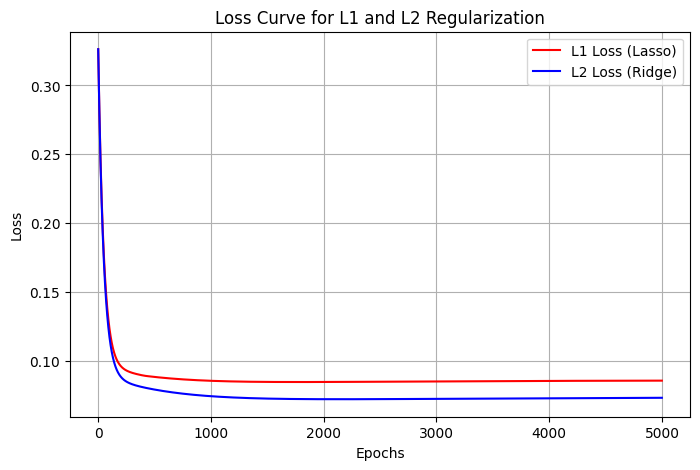
\includegraphics[width=0.7\textwidth]{cost_history.png}
    \caption{Cost function convergence for L1 and L2 regularization}
    \label{fig:cost_history}
\end{figure}


\section{Discussion on Regularization and Overfitting}

\begin{figure}[h]
    \centering
    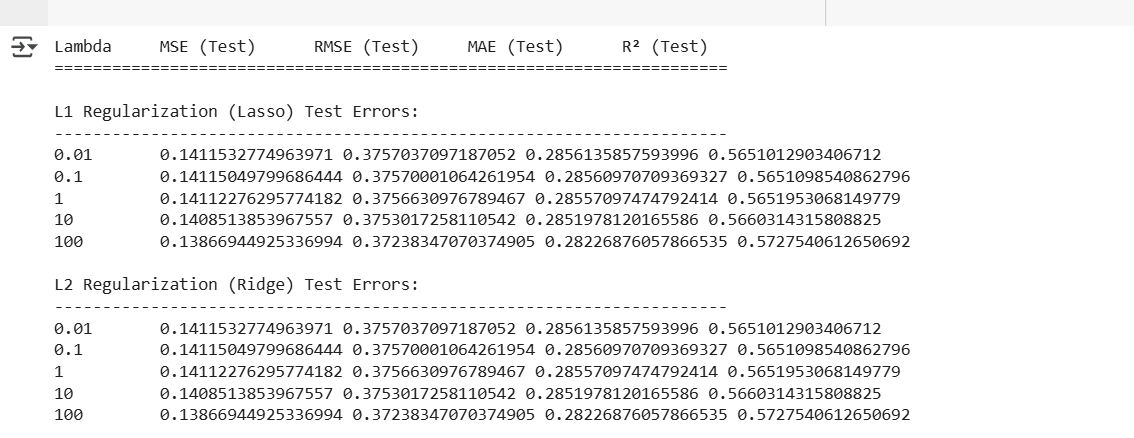
\includegraphics[width=0.7\textwidth]{diff_lambda.png} % Adjust width as needed
    \caption{Errors for different values of λ}
    \label{fig:diff_lambda}
\end{figure}

\subsection{Effect of L1 Regularization}
L1 regularization adds a penalty equal to the absolute value of the coefficients to the loss function. This approach encourages sparsity by driving some coefficients to zero, effectively performing feature selection. It's particularly useful when dealing with datasets containing many irrelevant or redundant features. However, this sparsity can lead to higher bias, as potentially informative features might be excluded from the model.

\subsection{Effect of L2 Regularization}
L2 regularization introduces a penalty proportional to the square of the coefficients. Unlike L1, it doesn't shrink coefficients to zero but rather distributes the weights more evenly, reducing the impact of any single feature. This method helps in reducing variance without significantly increasing bias, leading to a more balanced model. L2 regularization is especially effective when features are highly correlated.


\subsection{Overfitting and Regularization Strength}
The strength of regularization, controlled by the parameter 
λ, plays a crucial role in model performance:

!) Low λ Values: A small regularization strength allows the model to fit the training data closely, capturing noise and increasing the risk of overfitting.

2) High λ Values: A large regularization strength simplifies the model by heavily penalizing large coefficients, which may lead to underfitting and reduced predictive performance



\section{Conclusion}
\begin{itemize}
    \item Regularization techniques improve model generalization by reducing overfitting.
    \item L1 performs feature selection, while L2 stabilizes coefficient values.
    \item Gradient descent effectively optimizes these models for practical use.
    \item Future work can include experimenting with different regularization strengths (lambda values) and alternative optimization techniques.
\end{itemize}

\end{document}
